\documentclass[]{ximera}
%handout:  for handout version with no solutions or instructor notes
%handout,instructornotes:  for instructor version with just problems and notes, no solutions
%noinstructornotes:  shows only problem and solutions

%% handout
%% space
%% newpage
%% numbers
%% nooutcomes

%I added the commands here so that I would't have to keep looking them up
%\newcommand{\RR}{\mathbb R}
%\renewcommand{\d}{\,d}
%\newcommand{\dd}[2][]{\frac{d #1}{d #2}}
%\renewcommand{\l}{\ell}
%\newcommand{\ddx}{\frac{d}{dx}}
%\everymath{\displaystyle}
%\newcommand{\dfn}{\textbf}
%\newcommand{\eval}[1]{\bigg[ #1 \bigg]}

%\begin{image}
%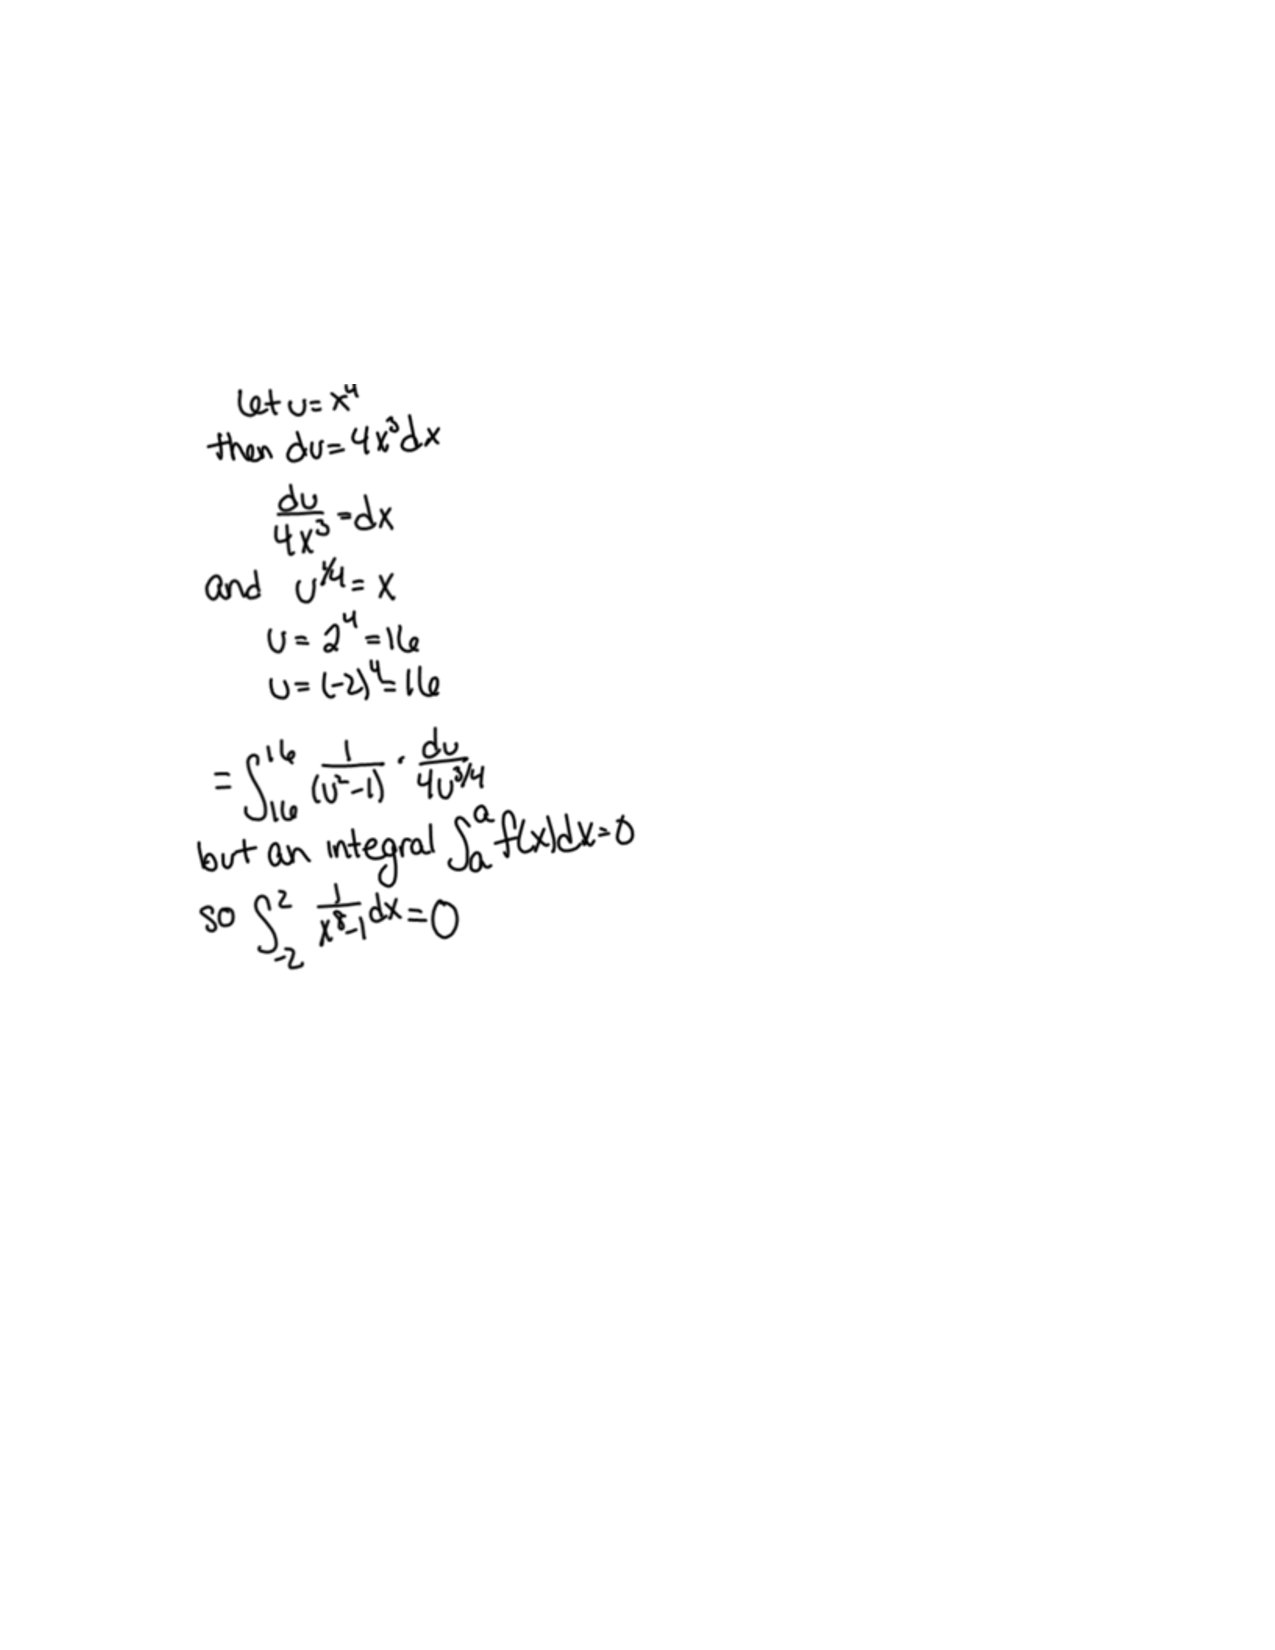
\includegraphics[trim= 170 420 250 180]{Figure1.pdf}
%\end{image}

%add a ``.'' below when used in a specific directory.
\newcommand{\RR}{\mathbb R}
\renewcommand{\d}{\,d}
\newcommand{\dd}[2][]{\frac{d #1}{d #2}}
\renewcommand{\l}{\ell}
\newcommand{\ddx}{\frac{d}{dx}}
\newcommand{\dfn}{\textbf}
\newcommand{\eval}[1]{\bigg[ #1 \bigg]}

\usepackage{multicol}

\renewenvironment{freeResponse}{
\ifhandout\setbox0\vbox\bgroup\else
\begin{trivlist}\item[\hskip \labelsep\bfseries Solution:\hspace{2ex}]
\fi}
{\ifhandout\egroup\else
\end{trivlist}
\fi} %% we can turn off input when making a master document

\title{Cross products}  

\begin{document}
\begin{abstract}		\end{abstract}
\maketitle



\section{Warm up:}
If $\vec{a}$, $\vec{b}$, and $\vec{c}$ are vectors in $3$-space $\mathbb{R}^3$, which of the following make sense?
	\begin{multicols}{3}
	\begin{enumerate}
	\item  $(\vec{a} \cdot \vec{b}) \cdot \vec{c}$
	\item  $(\vec{a} \cdot \vec{b})\vec{c}$
	\item  $(\vec{a} \times \vec{b}) \cdot \vec{c}$
	\item  $(\vec{a} \cdot \vec{b}) + \vec{c}$
	\item  $(\vec{a} \times \vec{b}) + \vec{c}$
	\item  $\vec{a} \cdot (\vec{b} + \vec{c})$
	\item  $\vec{a} \cdot (\vec{b} \times \vec{c})$
	\item  $\vec{a} \times (\vec{b} \cdot \vec{c})$
	\item  $(\vec{a} \times \vec{b}) \vec{c}$
	\end{enumerate}
	\end{multicols}
	
	\begin{freeResponse}
	\begin{enumerate}
	\item  Since $\vec{a} \cdot \vec{b}$ is a scalar, $(\vec{a} \cdot \vec{b}) \cdot \vec{c}$ does \dfn{not} make sense.
	\item  Now since $\vec{a} \cdot \vec{b}$ is a scalar, $(\vec{a} \cdot \vec{b})\vec{c}$ \dfn{does} make sense as regular scalar multiplication.
	\item  Since $\vec{a} \times \vec{b}$ is a vector, $(\vec{a} \times \vec{b}) \cdot \vec{c}$ \dfn{does} make sense.
	\item  This is of the form ``scalar + vector'', which does \dfn{not} make sense.
	\item  Since $\vec{a} \times \vec{b}$ is a vector, $(\vec{a} \times \vec{b}) + \vec{c}$ \dfn{does} make sense.
	\item  This is of the form ``vector $\cdot$ vector'', which \dfn{does} make sense.
	\item  This is also of the form ``vector $\cdot$ vector'', which \dfn{does} make sense.
	\item  This is of the form ``vector $\times$ scalar'', which does \dfn{not} make sense.
	\item  Since $\vec{a} \times \vec{b}$ is a vector, this does \dfn{not} make sense.
	\end{enumerate}
	\end{freeResponse}
	
\begin{instructorNotes}
This problem can be split up among the groups if the instructor likes (with maybe 3 or so per group).  
\end{instructorNotes}







\section{Group work:}



%problem 1
\begin{problem}
Given three dimensional vectors $\vec{u}$, $\vec{v}$, and $\vec{w}$, use dot product or cross product notation to describe the following vectors:
	\begin{enumerate}
	\item  The vector projection of $\vec{w}$ onto $\vec{u}$.
	
	\item  A vector orthogonal to both $\vec{u}$ and $\vec{v}$.
	
	\item  A vector with the length of $\vec{v}$ and the direction of $\vec{w}$.  
	
	\item  A vector orthogonal to $\vec{u} \times \vec{v}$ and $\vec{w}$.
	\end{enumerate}
	
	\begin{freeResponse}
	\begin{enumerate}
	\item  
		\[
		\text{proj}_u w = \boxed{\left( \frac{\vec{u} \cdot \vec{w}}{\vec{u} \cdot \vec{u}} \right) \vec{u}}
		\]
	
	\item  
		\[
		\boxed{\vec{u} \times \vec{v}}
		\]
	
	\item  
		\[
		\| \vec{v} \| \left( \frac{\vec{w}}{\| \vec{w} \|} \right) = \boxed{ \frac{\sqrt{\vec{v} \cdot \vec{v}}}{\sqrt{\vec{w} \cdot \vec{w}}} \vec{w}}
		\]
	
	\item  
		\[
		\boxed{(\vec{u} \times \vec{v}) \times \vec{w}}
		\]
	\end{enumerate}
	\end{freeResponse}
	
\end{problem}

\begin{instructorNotes}
This problem and the Warm-up are meant to force the students to make sense of scalar vs. vector quantities, as well as what quantities the dot and cross products produce.
\end{instructorNotes}







%problem 2
\begin{problem}
Find a vector of length $7$ that is perpendicular to both $\langle 5,-1,8 \rangle$ and $\langle -2,10,5 \rangle$.  
	\begin{freeResponse}
	Let $\vec{u} = \langle 5,-1,8 \rangle$ and $\vec{v} = \langle -2,10,5 \rangle$.
	Then a vector which is perpendicular to both $\vec{u}$ and $\vec{v}$ is $\vec{w} := \vec{u} \times \vec{v}$.  
	So we calculate
		\begin{align*}
		\vec{w} = \vec{u} \times \vec{v} = 
		\begin{vmatrix}
		\hat{\imath}	&	\hat{\jmath}	&	\hat{k}	\\
		5		&	-1		&	8		\\
		-2		&	10		&	5		\\
		\end{vmatrix}
		&= (-5 - 80) \hat{\imath} - (25 + 16) \hat{\jmath} + (50 - 2) \hat{k}  \\
		&= -85 \hat{\imath} -41 \hat{\jmath} + 48 \hat{k}
		\end{align*}
	A unit vector in the same direction as $\vec{w}$ is
		\[
		\frac{\vec{w}}{\| \vec{w} \|}
		= \frac{1}{\sqrt{(-85)^2 + (-41)^2 + 48^2}} \vec{w} = \frac{1}{\sqrt{11210}} \vec{w}.
		\]
	Therefore, a vector with a magnitude of $7$ in the same direction as $\vec{w}$ is
		\[
		\vec{t} = \frac{7}{\| \vec{w} \|} \vec{w} = \boxed{\frac{7}{\sqrt{11210}} \langle -85,-41,48 \rangle}
		\]
	\end{freeResponse}
		
\end{problem}

\begin{instructorNotes}

\end{instructorNotes}







%problem 3
\begin{problem}
A wrench that is $30$cm long lies along the positive $y$-axis and grips a bolt at the origin.  
A force is applied in the direction $\langle 0,3,-4 \rangle$ at the end of the wrench.  
Find the magnitude of the force needed to supply $100$J of torque to the bolt.
	\begin{freeResponse}
	Below is a picture of the situation
		
		%\begin{image}
		%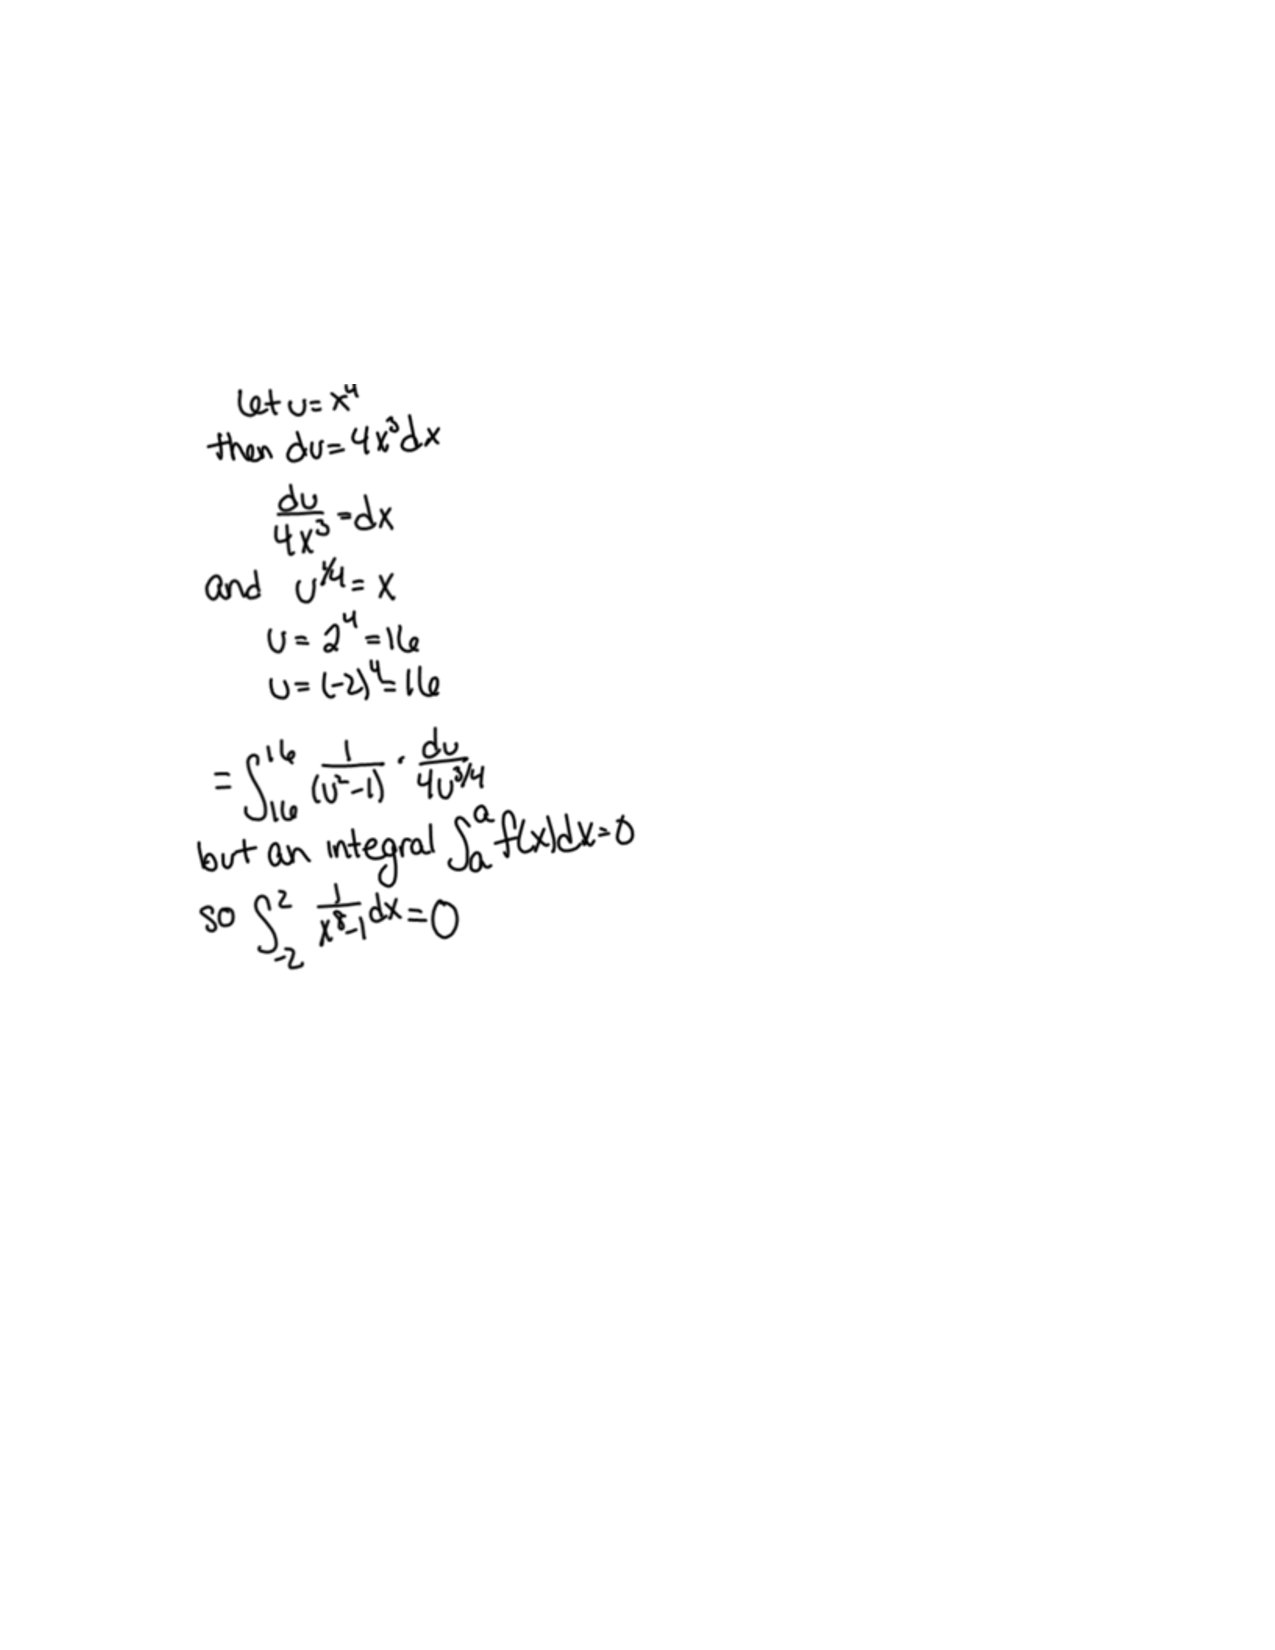
\includegraphics[trim= 170 220 170 180]{Figure1.pdf}
		%\end{image}
		
	Let
		\[
		\vec{R} = \langle 0, 0.3,0 \rangle 
		\]
	denote the position vector of the end of the wrench.  
	Since the force is in the direction $\langle 0,3,-4 \rangle$, we know that the force vector satisfies
		\[
		\vec{F} = c \, \langle 0,3,-4 \rangle = \langle 0, 3c, -4c \rangle
		\]
	for some constant $c$.
	Let $\vec{t}$ denote the torque vector.  
	Then $\vec{t} = \vec{R} \times \vec{F}$ and so $\| \vec{t} \| = \| \vec{R} \times \vec{F} \|$.
	Thus,
		\begin{align*}
		100 &= \| \langle 0,0.3,0 \rangle \times \langle 0,3c,-4c \rangle \|  \\
		&= 
		\biggr| \begin{vmatrix}
		\hat{\imath}	&	\hat{\jmath}	&	\hat{k}	\\
		0		&	0.3		&	0		\\
		0		&	3c		&	-4c		\\
		\end{vmatrix}  \biggr|  \\
		&= \| (-1.2c - 0) \hat{\imath} - (0-0) \hat{\jmath} + (0-0) \hat{k} \|  \\
		&= 1.2 c = \frac{6}{5} c.
		\end{align*}
	Therefore
		\[
		c = 100 \cdot \frac{5}{6} = \frac{500}{6} = \frac{250}{3}.
		\]
	So, the magnitude of the force is
		\begin{align*}
		\| \vec{F} \|
		&= \frac{250}{3} \sqrt{0^2 + 3^2 + (-4)^2}  \\
		&= \frac{250}{3} \cdot 5 = \boxed{\frac{1250}{3} \, N}
		\end{align*}
	\end{freeResponse}

\end{problem}

\begin{instructorNotes}
One goal in this problem is for students to make sense of the right-hand rule.  
The students need to know which direction of rotation tightens or loosens a bolt.  
\end{instructorNotes}
















	
	
	
	
	
	
	
	
	

	










								
				
				
	














\end{document} 


















